\documentclass[aps,showpacs,twocolumn,floats,prd,superscriptaddress,nofootinbib]{revtex4-1} 
\usepackage{graphicx,amsmath,amssymb,amstext}
\usepackage{amssymb,amsbsy,amsfonts,amsthm,color}
\usepackage{epsfig}
%\usepackage{showkeys}
\usepackage{graphicx}
\usepackage{subfigure}
\usepackage{sidecap}
\usepackage{floatrow}
\graphicspath{{Figures/}}

\begin{document}

\title{A self-consistency check for the unitary propagation of Hawking quanta}

\author{Daniel Baker}
\email{dbaker@cita.utoronto.ca}
\affiliation{Canadian Institute of Theoretical Astrophysics, 60 St George St, Toronto, ON M5S 3H8, Canada.}
\affiliation{University of Toronto, Department of Physics, 60 St George St, Toronto, ON M5S 3H8, Canada.}

\author{Darsh Kodwani}
\email{dkodwani@physics.utoronto.ca}
\affiliation{Canadian Institute of Theoretical Astrophysics, 60 St George St, Toronto, ON M5S 3H8, Canada.}
\affiliation{University of Toronto, Department of Physics, 60 St George St, Toronto, ON M5S 3H8, Canada.}

\author{Ue-Li Pen}
\email{pen@cita.utoronto.ca}
\affiliation{Canadian Institute of Theoretical Astrophysics, 60 St George St, Toronto, ON M5S 3H8, Canada.}
\affiliation{Canadian Institute for Advanced Research, CIFAR program in Gravitation and Cosmology.}
\affiliation{Dunlap Institute for Astronomy \& Astrophysics, University of Toronto, AB 120-50 St. George Street, Toronto, ON M5S 3H4, Canada.}
\affiliation{Perimeter Institute of Theoretical Physics, 31 Caroline Street North, Waterloo, ON N2L 2Y5, Canada.}

\author{I-Sheng Yang}

\email{isheng.yang@gmail.com}
\affiliation{Canadian Institute of Theoretical Astrophysics, 60 St George St, Toronto, ON M5S 3H8, Canada.}
\affiliation{Perimeter Institute of Theoretical Physics, 31 Caroline Street North, Waterloo, ON N2L 2Y5, Canada.}

\begin{abstract}
The black hole information paradox presumes that local quantum field theory is valid to provide unitary propagations from near-horizon modes to asymptotic Hawking quanta. 
Instead of invoking unknown quantum-gravity effects to modify such assumption, we propose a self-consistency check.
We re-examine this assumption by establishing an analogy to Feynman's analysis of a double-slit experiment. 
Feynmann showed that the assumption of subsystem unitarity in double-slit experiment, namely ignoring the entanglement with the double-slit, becomes arbitrarily reliable when the screen to project the interference pattern goes to infinitely far away.
Analogously, here we ask whether a unitary propagation of Hawking quanta, namely ignoring the entanglement with the geometry, also becomes arbitrarily reliable in the limit of a large black hole. 
We present strong evidence that the result is negative, and we discuss its implications.
\end{abstract}

\maketitle


\onecolumngrid

\section{Introduction and Summary}

Quantum mechanical evolution of a full system is by-definition unitary. 
Unfortunately, we are not always able to describe everything by quantum mechanics all together. 
Practical descriptions are always about subsystems. 
Namely, we assume that the full system can be separated into a ``classical background'' and a ``quantum subsystem''. 
Since we only use quantum mechanics to describe the quantum subsystem, it always appears to be unitary.
\footnote{Even a time-dependent Hamiltonian leads to an apparently unitary evolution under this assumption. That is obviously not a physical fact since a unitary subsystem should be determined by its own initial state, not co-determined by initial state plus an arbitrary time-dependence.} 
However, such unitarity should not be taken as a physical fact unless one specifically checks the nature of interactions with the background.

The most direct way to justify the classical-background assumption is to also describe the background in quantum mechanics, and verify that the quantum interaction between the background and the quantum subsystem indeed does not entangle them. 
This is clearly difficult in practice. 
The very reason why we would like to apply the classical-background approximation is to avoid describing the far-too-complicated background by quantum mechanics. 
A consistency check which requires us to do so defeats the purpose. 
Furthermore, there are situations in which we in-principle do not know how to describe the classical background in quantum mechanics. 
Quantum field theory in curved spacetime is a perfect example. 
In this case, the classical background is the geometry.
One in-principle needs to know quantum gravity in order to model the quantum interaction with the background. 

Fortunately, Feynman, in his famous lectures, presented an interesting trick to circumvent the above obstacle. 
This trick, to a certain extend, enables us to perform a self-consistency check of the classical-background assumption {\bf without} knowing the quantum nature of the background.
In Sec.\ref{sec-DoubleSlit}, we will review Feynman's analysis on the double-slit experiment. 
In his case, the double-slit is the classical background, the particle passing through it is the quantum subsystem, and the operational definition of subsystem unitarity is whether an interference pattern can be observed on the final projection screen. 
He showed that we can ignore the quantum details of the double-slits and summarize that as an uncertainty in its position, which is a classical quantity. 
When such uncertainty is fixed, the interference pattern is always visible as long as we put the final projection screen to be infinitely far away. 
It is in this sense that a unitary evolution of the subsystem is an arbitrarily good approximation.

The fundamental principle from Feynman's trick is that ``classical wave coherence'' should be taken as the prerequisit of ``quantum unitarity''. 
In Sec.\ref{sec-QFT}, we argue that it has a natural generalization to local QFT in curved spacetime, thus we can apply it to re-examine the propagation of Hawking quanta. 
This propagation is of particular importance because it plays a central role in the lasting debate of black hole information paradox. 
The main dilemma is that one Hawking quantum needs to play two different roles. 
Near the horizon, it has to be part of the local vacuum state; near spatial infinity, it has to recover a unitary evaporation process. 
For an old black hole, the same state of a Hawking quantum cannot fulfill both requirements, thus the paradox. 
If the propagation process from near the horizon to infinity is not unitary, then a near horizon mode and the asymptotic Hawking quantum does not have the same state, and the paradox loses its fundation. 
Thus before jumping into any conclusion regarding the paradox, we should try to confirm whether QFT in a curved spacetime is indeed justified to provide a unitary propagation of Hawking quanta.

In Sec.\ref{sec-BlackHole}, we will provide our detail analysis and analogy. 
Roughly speaking, the classical geometry plays the role of the double-slit, a background that can potentially entangle with the Hawking quanta wavefunction and ruins its subsystem unitarity. 
We then assume that the unknown quantum nature of geometry can be parametrize by a classical uncertainty with an unknown but fixed, gauge-invariant size. 
A classical wave plays the role of the interference pattern; if even a classical wave decoheres due to the uncertainty of geometry, there is no reason to believed that the quantized version of such wave has unitarity.
The common belief is that in the limit of a large black hole, gravitational effect outside the horizon is arbitrarily weak, thus local QFT should be arbitrarily trustworthy.
By analogy to Feynman's analysis, we should expect that with a fixed uncertainty in the geometry, any effect on the classical wave should drops to zero when we take the large black hole limit.
Interestingly, what we found seems to be the opposite. 
We show that with a fixed geometric uncertainty, a classical wave suffers an {\it arbitrarily large} correction in the large black hole limit.
By analogy to Feynman's analysis, this as a strong evidence that the apparent unitarity of QFT in this case is not a valid assumption.

{\bf XXX tbc by I-Sheng}


\section{Feyman's analysis on double-slit experiments}
\label{sec-DoubleSlit}

Double-slit interference is the signature experiment to demonstrate the nature of quantum mechanics. Figure 1 shows a simple example of such experiment.
When a group of particles of the same momentum pass through slit 1 only, they reach the final screen as some probability distribution $P_1(y)$. 
When they pass through slit 2 only, they reach the final screen as a probability distribution $P_2(y)$.
When both slits are open, the probability distribution we find on the final screen is not a simple sum; $P_{12}(y) \neq P_1(y) + P_2(y)$! 
Instead, the final screen shows an interference pattern which can only be explained by wavefunctions.
$P_i = \langle \phi_i | \phi_i \rangle$ and $P_{12} = (\langle \phi_1|+\langle \phi_2| ) (|\phi_1\rangle + | \phi_2 \rangle)=P_1 + P_2 + 2{\rm Re}\langle\phi_1|\phi_2\rangle$.

\ \\ \ \\
{\bf XXX insert the double-slit figure here: Darsh.}
\ \\ \ \\

This standard explanation works because we assume the particle is the only quantum-mechanical system here, and it can be describe by a pure state, $|\phi\rangle_{\rm particle} = |\phi_1\rangle + |\phi_2\rangle$.
But if quantum mechanics is correct, this particle is not the only thing to be described by a wavefunction. 
For example, we can also describe the double-slit by its wavefunction $|\psi\rangle_{\rm ds}$. The total wavefunction of the combined system can be in a pure state,
\begin{equation}
|\Psi\rangle_{\rm combined} = |\psi_1\rangle_{\rm ds}|\phi_1\rangle_{\rm particle} 
+ |\psi_2\rangle_{\rm ds}|\phi_2\rangle_{\rm particle} ~,
\end{equation}
but either subsystem does not have to be pure.

When the two double-slit states are almost indistinguishable,
\begin{equation}
\langle\psi_1|\psi_2\rangle\langle\psi_2|\psi_1\rangle \approx 1~,
\label{eq-pure}
\end{equation}
then the combined system factorizes,
\begin{equation}
|\Psi\rangle_{\rm combined} \approx |\psi_1\rangle_{\rm ds}
\left(|\phi_1\rangle_{\rm particle} + |\phi_2\rangle_{\rm particle}\right) ~.
\end{equation}
The particle subsystem indeed stays as a pure state and there will be an interference pattern.

On the other hand, if the two double-slit states are distinguishable,
\begin{equation}
\langle\psi_1|\psi_2\rangle\langle\psi_2|\psi_1\rangle \ll 1~,
\label{eq-mixed}
\end{equation}
that means the interaction entangled the two systems. The particle subsystem becomes a mixed state,
\begin{equation}
\rho_{\rm particle} = {\rm Tr}_{\rm ds}|\Psi\rangle\langle\Psi| \approx
|\phi_1\rangle\langle\phi_1| + |\phi_2\rangle\langle\phi_2|~,
\end{equation}
and there will be no interference pattern.

Whether the double-slit states are given by Eq.~(\ref{eq-pure}) or (\ref{eq-mixed}) seems to require the knowledge about the actual quantum-mechanical interacton between the particles and the double-slit, which is unavailable in practice.
Feynman pushed the above analysis further to overcome such problem.
He pointed out that even if we try to keep the interaction minimal, there will be one inevitable interaction that makes $|\psi_1\rangle$ and $|\psi_2\rangle$ different.
That is because when a particle reaches some place on the screen, its $y$-momentum must be different depending on which slit it passed through.
\begin{equation}
\Delta p_y^{\rm particle} \equiv 
|\langle\phi_1|p_y|\phi_1\rangle - \langle\phi_2|p_y|\phi_2\rangle| 
\approx p_x \frac{s}{L}~,
\end{equation}
where $p_x$ is the $x$ momentum of the particles, $s$ is the separation between the two slits, and $L$ is the distance to the screen. 
This means two different values of recoil momentum on the double-slit,
\begin{equation}
\Delta p_y^{\rm ds} = \Delta p_y^{\rm particle} \approx p_x \frac{s}{L}~.
\label{eq-dpds}
\end{equation}
The uncertainty principle sets a limit on how well we can measure this difference. Namely, we need a large uncertainty in the position to measure a small change in momentum. Setting $\hbar$ to 1, we can say that when the momentum difference is too small to be measured,
\begin{equation}
\Delta p_y^{\rm ds} < 1/\Delta y^{\rm ds}~,
\label{eq-standard}
\end{equation} 
then Eq.~(\ref{eq-pure}) is true and the two states are indistinguishable. 
Otherwise Eq.~(\ref{eq-mixed}) is true and the two states are distinguishable.

The key point is that there is an alternative way to appreciate Eq.~(\ref{eq-standard}) {\it without} thinking about the quantum mechanics of the double-slit. 
First of all, the interference pattern has a fringe width of  
\begin{equation}
w = L\frac{\lambda}{s}~,
\end{equation}
where $\lambda = p_x^{-1}$ is the de Broglie wavelength of the particle. This is the separation of bright/dark lines in the $y$ direction with a fixed reference point at the $y$ position of the double-slit. Thus the uncertainty in the $y$ position must be smaller than this value, so the interference pattern is not totally blurred.
\begin{equation}
\Delta y^{\rm ds} < w = \frac{L}{p_xs}~.
\label{eq-stdcls}
\end{equation}
This is exactly the same condition as in Eq.~(\ref{eq-standard}).

We should emphasize the key value of this result. We can treat both the position uncertainty $\Delta y^{\rm ds}$ and the interference fringe width $w$ as classical quantities. Eq.~(\ref{eq-stdcls}) is then a purely classical calculation to compare these two quantities, which tells us whether a classical wave pattern (the intereference pattern) loses coherence. If we only take its face value, it seems to be only a practical obstacle of measuring the interference pattern. One might argue that the underlying subsystem unitarity is still valid, just difficult to measure. 

What Feynman showed by this example is that Eq.~(\ref{eq-stdcls}) tells us exactly the same thing as Eq.~(\ref{eq-standard}). The later {\bf is} directly about quantum mechanics and shows how the subsystem unitarity can fail. Thus an apparently classical calculation can tell us something about the hidden quantum-mechanical nature of the interaction between the double-slit and the particle passing through it. In this example, it tells us whether the particles get entangled with the double-slit and loses its subsystem unitarity. 

One might object that the above analysis is only applicable if we are {\it given} a particular value of $\Delta y^{\rm ds}$, while in fact such quantity has to originate from the unknown quantum mechanics of the double-slit. This is a valid concern, and it actually shows another strength of Eq.~(\ref{eq-stdcls}). Indeed we do not know the value of $\Delta y^{\rm ds}$ just from classical physics, but it is very reasonable to assume that it is intrinsic to the double-slit. Namely, its value should be fixed if we move the screen further away. Eq.~(\ref{eq-stdcls}) shows that with a fixed $\Delta y^{\rm ds}$, we can always make $L$ large enough to satisfy this condition. Thus, at least at the level of gedanken experiment, one can always arrange a situation that the interference pattern is visible, thus the subsystem unitarity is valid.

\section{Analogy in Quantum Field Theory}
\label{sec-QFT}

The double-slit interference is an example that both the classical coherence and quantum unitarity can be calculated explicitly and show that they follow the same condition.
Here, we advocate that such relation is actually a general rule.
{\it Classical coherence, instead of thinking it as a practically of measurements, should be treated as a prerequisit to quantum unitarity.} 
Thus when classical coherence fails, not only have we no practical measurements to confirm the purely of the subsystem wavefunction, such wavefunction {\it actually did not evolve unitarily.}
Whatever effect responsible for a classsical uncertainty large enough to disrupt classical coherence must have also interacted with the subsystem quantum-mechanically and became entangled with it.

For quantum field theory in a curved spacetime, we always assume that the quantum fields is a subsystem that never entangles with the geometry, thus remains unitary.
Since we do not know quantum gravity/geometry, we cannot directly check this assumption by an actual calculation of entanglement.
However, we can always check classical coherence, and by this rule we advocate, the answer directly prove/disprove subsystem unitarity.

If we go back to the basic of quantum field theory, this new rule we advocate makes a lot of sense. As shown in Fig.\ref{fig-QFT}, QFT starts from solving a classical mode function, then quantizing its amplitude into a quantum state. 
Any method to measure such quantum state assumes the knowledge of the classical mode function. 
If the geometric uncertainty leads to an order one change in the classical mode function, then there is no practical way to reliably measure its quantum state. 
We advocate that this is not only a practicality about measuring the quantum state, but it directly tells us that the quantum state loses its unitarity. 
Just like in Feynman's example where the uncertainty of the double-slit guarantees its entanglement with the particles, whatever effect that leads to the geometric uncertainty here must entangle with the quantum state of this mode. 
Without a theory of quantum geometry, we cannot describe how that happens. 
But through a classical calculation, we can determine whether it has happened or not.

\ \\ \ \\
{\bf XXX insert the QFT figure here: Darsh or I-Sheng}


\section{Hawking quanta propagation}
\label{sec-BlackHole}

The usual treatment of how a near-horizon mode becomes an asymptotic Hawking quantum is also following a fixed-background assumption.
The background is the Schwarzschild geometry.
\begin{equation}
ds^2 = -\left(1-\frac{2M}{r}\right)dt^2 + \frac{dr^2}{1-\frac{2M}{r}} + r^2d\Omega_2^2~.
\end{equation}
When one applies local quantum field theory to describe a field on this fixed background, the result is by-definition unitary, but that is not necessary a physical fact. 
Given how little we understand quantum gravity, a classical self-consistency check as we described in the previous section is a reasonable thing to do.

\subsection{Setup and summary}

\begin{itemize}
\item {\bf Classical coherence by tracking geodesics.} The classical mode of a massless field basically has its peaks and nodes following null geodesics.
Thus, instead of actually solving the mode function, we can perform a much simpler calculation to track geodesics.
We start with two out-going null geodesics with the separation of one period of such mode near the horizon, and then we calculate the change in their separations at spatial infinity.
If such change is comparable to the wavelength, then the mode function of this wavelength loses classical coherence.
\item {\bf The background and the uncertainty.} The classical background in this case is the Schwarzschild geometry, which can be written as the metric $g_{\mu\nu}$. 
A classical uncertainty can be expressed as deviation from such metric, $\Delta g_{\mu\nu}$. 
There are two major challenges here.
\begin{enumerate}
\item There are many more variables than the double-slit experiment. 
We consider only one particular form of $\Delta g_{\mu\nu}$ in this paper---back-reactions from the presence of extra matter of zero total energy. 
It is simple to calculate and reflects the physcial intuition of vacuum pair fluctuation.
\item The value of $\Delta g_{\mu\nu}$ is gauge dependent. 
By relating it to the presence of extra matter, we can express it to a gauge-invariant local quantity, which is the natural thing to hold fixed in our analysis.
\end{enumerate}
Note that if we were reporting a positive result, that such uncertainty upholds unitarity, then one should question the validaty of learning a general lesson from a special example. However, we will show that this particular form of $\Delta g_{\mu\nu}$ is already sufficient to question unitarity, and we did not choose this form to specifically do that. Thus our limited analysis is sufficient to raise a reasonable doubt to the classical-background approximation.
\item {\bf Renormalization.} It is well-known that na\"ive applications of QFT often suffer from UV/IR divergences.
In our case, we will see that even in Minkowski space, geometric uncertainty already leads to a finite change between the two null geodesics.
We will simply ``renormalize'' that away by saying that if the black hole case leads to a similar change, it should not be taken as a serious problem.
Our surprising result is that in the black hole case, we get an infinitely larger change, which is difficult to blame on renormalization.
\end{itemize}

More concretely, our setup is like in Fig.\ref{fig-setup}. 
We start by choosing two points at some $r_0\gg M$ with a $\delta t_0\sim M$ coordinate time separation between them.
This represents one wavelength of the mode function of an asymptotic Hawking quantum.
We then back-track two null geodesics from these two points back to two points near the horizon, at $r_A$ with $(r_A-2M)\ll 2M$.
Now their separation represents one wavelength of a near-horizon mode, which would have propagated to the asymptotic mode if there were no geometric uncertainty. 
We then introduce introduce a geometric uncertainty as two shells of zero total ADM mass. 
Therefore, both the near horizon and the asymptotic regions are not affected by such uncertainty.
Only the process of propagation is affected.
With the same two starting points near the horizon. we calculate the separation $\bar{\delta t_0}$ of the two null geodesics when they arrive at $r_0$, and compare it with $\delta t_0$.

\begin{figure}[tb]
\begin{center}
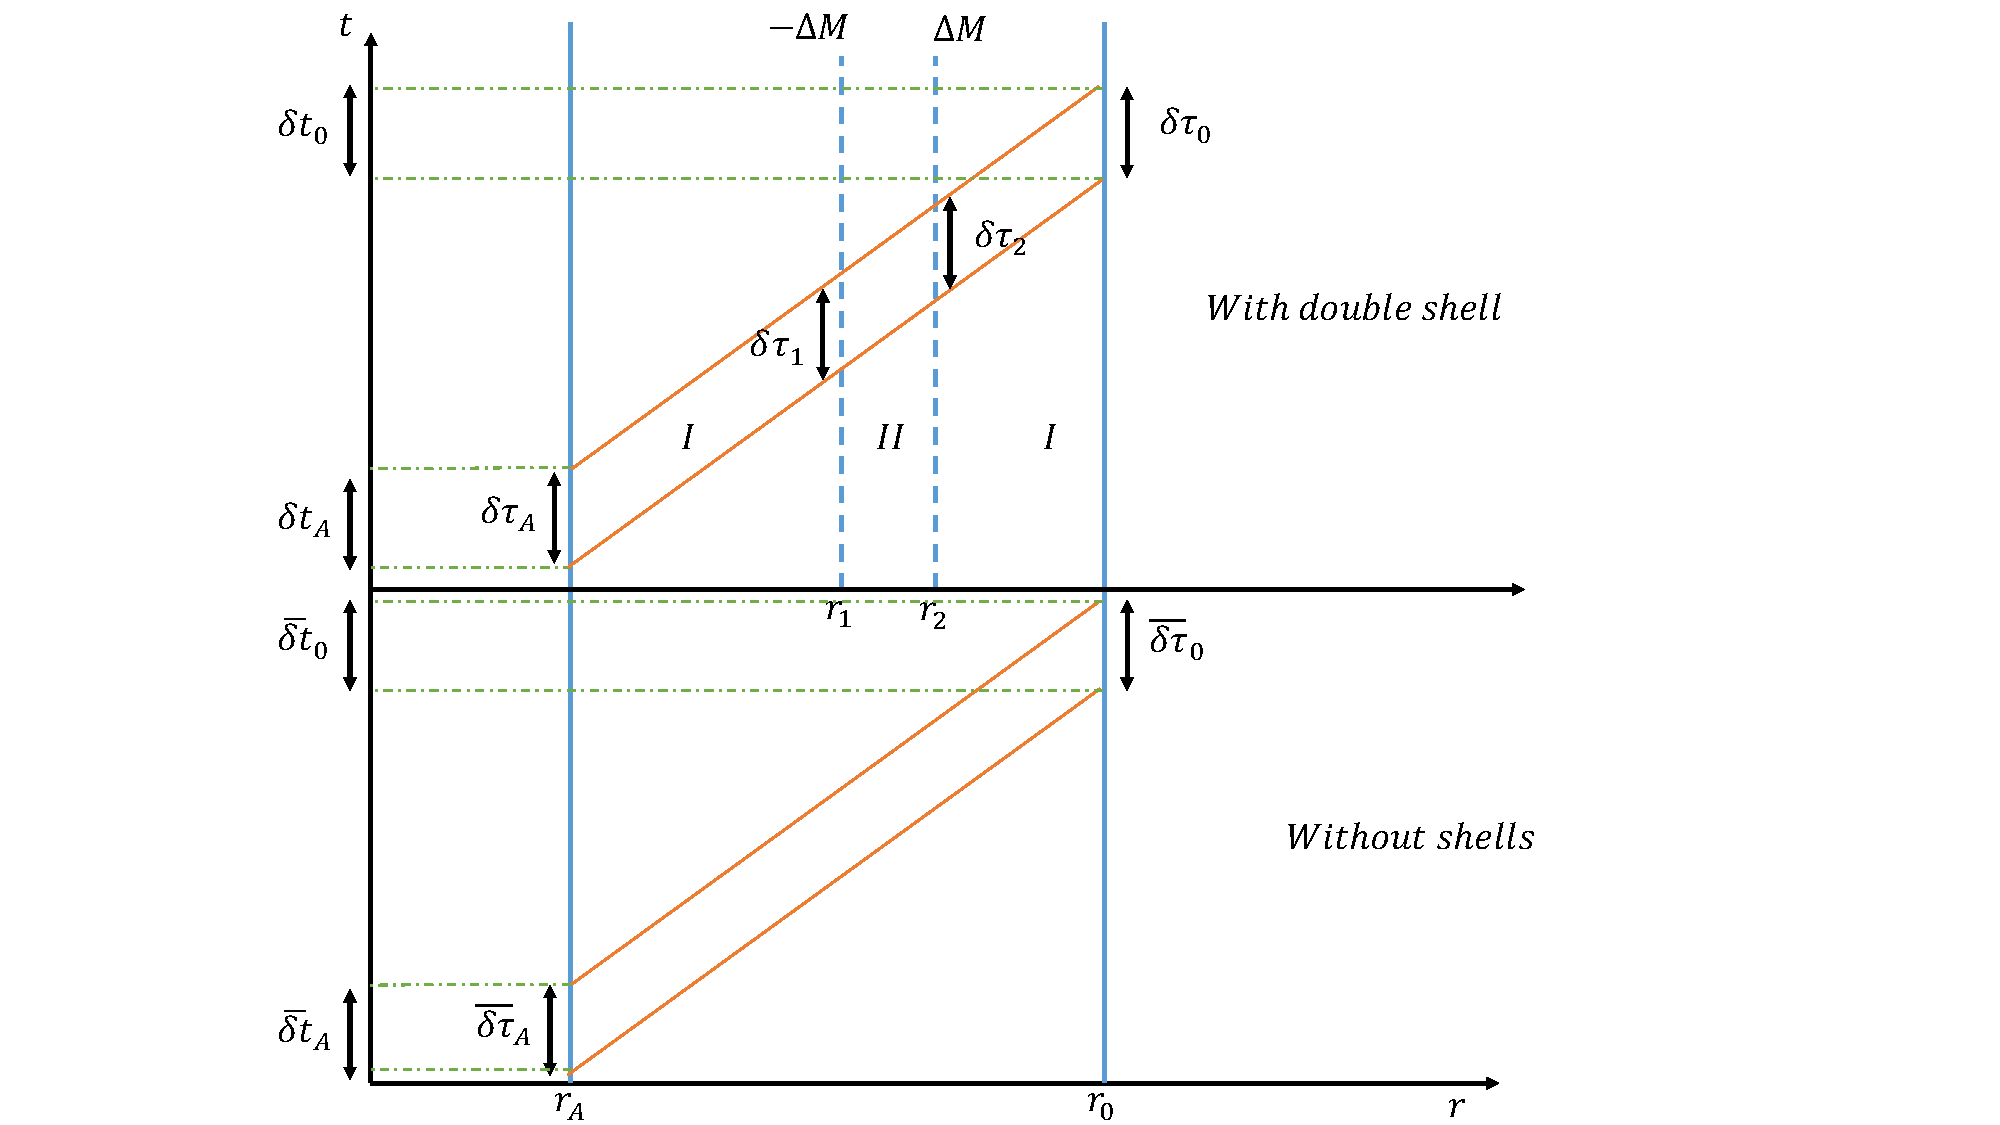
\includegraphics[scale = 0.6]{Propertime.pdf}
\caption{The two parts of this diagrams describe two different scenarios. The trajectories of the photon are the lines in orange. The trajectory of the observer and the position from which the photons are emitted are represented by solid blue lines. The bottom part is a general case of two Hawking photons coming from a distance $r_A$ from the black hole of mass $M$ and arriving at an observer who is at a distance of $r_0$. The top part shows two Hawking photons coming from the same distance $r_A$ from a black hole of mass $M$. Instead of the photons freely propagating through to an observer at $r_0$, they have to cross two shells, represented by blue dotted line, of equal and opposite mass $-\Delta M, \Delta M$ at $r_{1}, r_{2}$ respectively. The regions $I$ represent a metric with mass $M$ and region $II$ represents a metric with mass $M-\Delta M$.}
\label{fig-setup}
\end{center}
\end{figure}

After some formal calculations in the {\bf Appendix}, we arrive at this simple expression:
\begin{equation}
\frac{\delta t_0 - \bar{\delta t_0}}{\delta t_0} = 
\left(\sqrt{\frac{r_2-2M}{r_1-2M}}\sqrt{\frac{r_1-2(M-\Delta M)}{r_2-2(M-\Delta M)}}-1\right)~,
\label{eq-result}
\end{equation}
where $r_1$ is the location of the inner shell, $r_2$ is the location of the outer shell, and $\pm\Delta M$ are their individual ADM masses.

\subsection{Physical interpretation}

As the first step, we set $M=0$ in Eq.~(\ref{eq-result}) to study its meaning in Minkowski space. Assuming that $|r_1-r_2| \equiv \Delta r \ll r_1$ and $\Delta M \ll r_1$, the leading order result becomes
\begin{equation}
\frac{\delta t_0 - \bar{\delta t_0}}{\delta t_0} \approx \frac{\Delta M}{r_1^2} \Delta r 
\equiv \sigma \Delta r~.
\label{eq-Mink}
\end{equation}
This seems to be a reasonable answer. 
First of all, it is quite unlikely that the entire shell of mass $\Delta M$ fluctuates out of vacuum.
It is reasonable that any change to the null geodesics is about a local energy density of the particular piece of shell they happen to pass through.
Secondly, this result is gauge invariant. For an observer at rest, $\sigma$ is the local energy density and $\Delta r$ is the proper distance. 
For a boosted observer, $\sigma$ increases by a boost factor while $\Delta r$ contracts by the same factor.
We take it as a good sign that other forms of geometric uncertainty can also be parametrize by a similar, gauge invariant quantity.

The na\"ive interpretation of Eq.~(\ref{eq-Mink}) is that even in Minkowski space, geometric uncertainty can potentially decohere classical mode functions.
By our definition, that poses some threat to QFT in Minkowski space.
We are going to assume that unitarity in QFT is fine in Minkowski space, effectively ``renormalize away'' the effect of Eq.~(\ref{eq-Mink}).
One can imagine a simple subtraction by a counter term.
Or alternatively, since the actual value of $(\sigma\Delta r)$ is unknown, we assume that it is small enough to not cause any concern.

Next we study Eq.~(\ref{eq-result}) with an actual black hole. When the double-shell is very far away from the black hole, $r_1\gg M$, it agrees with Eq.~(\ref{eq-Mink}) as expected. The interesting thing here is that when this pair of geodesics originate near the horizon, the double-shell could also be somewhere near the horizon. In that limit, Eq.~(\ref{eq-result}) can be approximated by
\begin{equation}
\frac{\delta t_0 - \bar{\delta t_0}}{\delta t_0} \approx
\sigma \Delta l \left(\frac{2M}{l_1}\right)^2~, \ \ \ \ {\rm \bf XXX \ check \ coefficients}
\label{eq-NearHorizon}
\end{equation}
where $l$ is the proper distance between $r_1$ and the horizon and $\Delta l$ is the proper distance between the two shells. We can see that in addition to the same gauge-invariant quantity in Minkowski space\footnote{In Minkowski space, the radial coordinate is the proper distance, $\Delta r=\Delta l$.}, there is an extra factor of $(2M/l_1)^2$ which diverges as the shell approaches the horizon.

The small $l_1$ limit may not be the best way to appreciate how Eq.~(\ref{eq-NearHorizon}) poses a threat to QFT. After all, we do not expect QFT to hold for arbitrarily small distance anyway. The best way to understand Eq.~(\ref{eq-NearHorizon}) is to fix $l_1$ at some scale that much longer than any scale that we expect UV problems. By conventional knowledge, the effect of gravity near horizon gets arbitrarily weak as the black hole becomes large. However, the problem caused by Eq.~(\ref{eq-NearHorizon}) grows larger as the black hole becomes larger, and diverges in the large black hole limit.


\section{Discussion}

{\bf XXX Maybe do this in the introduction: I-Sheng.}

\appendix


\section{Calculation}

{\bf XXX Modify the content accordingly to fit their status in the appendix: Darsh/Daniel.}

\subsection{Proper time}

\subsubsection{Background spacetime}

First we consider the motion of Hawking photons coming from a Schwarzschild metric of the form

\begin{equation}
	ds^2 = - \left( 1 - \frac{2M}{r} \right) dt^2 + \left( 1 - \frac{2M}{r} \right)^{-1} dr^2 + r^2 d \Omega_2^2.
\end{equation}

Consider two Hawking photons coming from a fixed distance, $r_{e}$, just above a Schwarzschild black hole separated by a coordinate time interval $\bar{\delta t}_A$ and a corresponding proper time $\bar{\delta \tau}_A$ as shown in figure \ref{fig:1}. The two photons propagate through to the observer at $r_0$ following geodesics. We could potentially solve for the geodesics of the photons to find out the coordinate time of arrival of each photon, however in the absence of additional gravitational fields the coordinate time interval between the photons will not change\footnote{This will prove to be extremely helpful when we look at the calculation in the presence of shells.}, i.e $\bar{\delta t}_A = \bar{\delta t}_0$, and that is the quantity we need in order to compute the proper time $\bar{\delta \tau}_0$ observed by the observer at $r_0$,

\begin{eqnarray}
	\bar{\delta \tau}_0 & = & \left( 1- \frac{2M}{r_0} \right)^\frac{1}{2} \bar{\delta t}_0	\nonumber	\\
	& = & \left( 1 - \frac{2M}{r_0} \right)^\frac{1}{2} \bar{\delta t}_A \approx \bar{\delta t}_{A} 
\end{eqnarray}

where in the last step we have assumed $r_0$ is very large.

\subsubsection{Introducing perturbations: Double shells}


\begin{figure}[h!]
\begin{center}
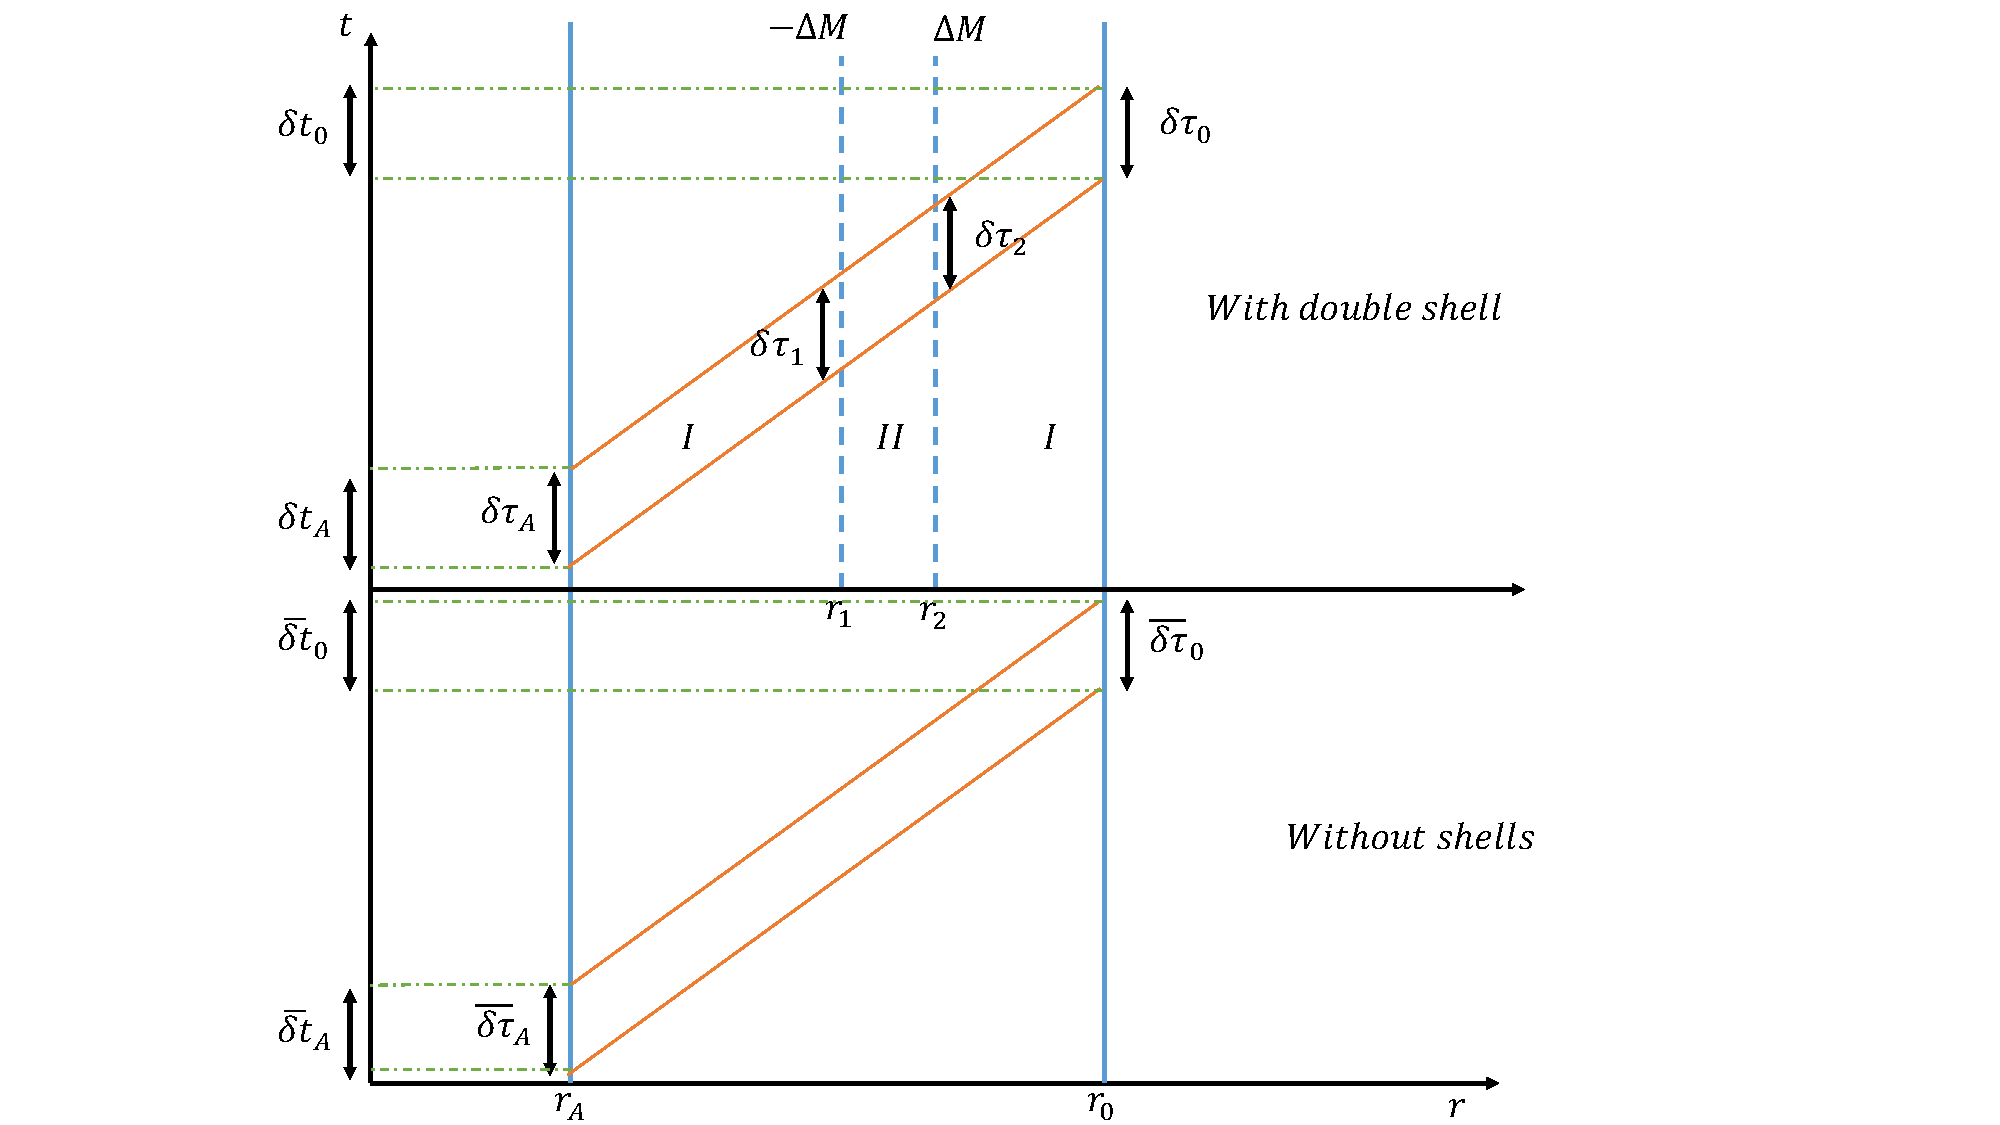
\includegraphics[scale = 0.6]{Propertime.pdf}
\caption{The two parts of this diagrams describe two different scenarios. The trajectories of the photon are the lines in orange. The trajectory of the observer and the position from which the photons are emitted are represented by solid blue lines. The bottom part is a general case of two Hawking photons coming from a distance $r_A$ from the black hole of mass $M$ and arriving at an observer who is at a distance of $r_0$. The top part shows two Hawking photons coming from the same distance $r_A$ from a black hole of mass $M$. Instead of the photons freely propagating through to an observer at $r_0$, they have to cross two shells, represented by blue dotted line, of equal and opposite mass $-\Delta M, \Delta M$ at $r_{1}, r_{2}$ respectively. The regions $I$ represent a metric with mass $M$ and region $II$ represents a metric with mass $M-\Delta M$.}
\label{fig:1}
\end{center}
\end{figure}


In this section we consider the top part of figure \ref{fig:1}. To distinguish the results from the previous section without shell we will not have an overbar in any of the quantities described in this scenario. The same initial conditions for the two Hawking photons are assumed. Using the argument described in the previous section we expect the coordinate time intervals between $r_A$ and $r_1$ to be equal, $\delta t_A = \delta t_1$. Analogously for the coordinate time interval between $r_2$ and $r_0$, $\delta t_2 = \delta t_0$. The new region is between $r_2$ and $r_1$ where the metric is different; it is defined by a mass $M - \Delta M$. The coordinate time interval at $r_1$ will also have a representation in the $II$ metric. Quantities evaluated in the $II$ metric will be denoted by a hat on top. By imposing the physical condition that there cannot be any discontinuities in spacetime we know that the proper times in both the metrics must be the same at $r_1$, $\delta \tau_1 = \delta \hat{\tau}_1$ and this gives a relation between the coordinate time intervals

\begin{equation}
	\delta t_1 = \left( \frac{1 - \frac{ 2(\Delta M -M)}{r_1})}{1 - \frac{ 2M}{r_1}}  \right)^\frac{1}{2} \delta \hat{t}_1.	\label{shell1}
\end{equation}

Applying the same condition to the proper times at $r_2$ gives the analogous relation between the coordinate time intervals at $r_2$, 

\begin{equation}
	\delta t_2 = \left( \frac{1 - \frac{ 2(\Delta M -M)}{r_2})}{1 - \frac{ 2M}{r_2}}  \right)^\frac{1}{2} \delta \hat{t}_2. 	\label{shell2}
\end{equation}

Since $\delta \hat{t}_1$ and $\delta \hat{t}_2$ are both evaluated in the same metric they must be equal and therefore we can combine Eq (\ref{shell1}) and Eq (\ref{shell2}) to give a relation between $\delta t_1$ and $\delta t_2$, 

\begin{eqnarray}
	\delta t_{1} & = & \left( \frac{ \left( 1 - \frac{2 M - \Delta M}{r_{1}} \right) \left( \frac{1 - 2M}{r_{2}} \right)}{\left( 1 - \frac{2M}{r_{1}} \right)  \left( 1 - \frac{2(M - \Delta M)}{r_{2}} \right)} \right)^\frac{1}{2} \delta t_{2}	\nonumber	\\
	& = & \left( \frac{2M - r_2}{2M - r_1} \right)^\frac{1}{2} \left( \frac{ 2(\Delta M - M) + r_1}{2(\Delta M - M) + r_2} \right)^\frac{1}{2} \delta {t}_{2}.
\end{eqnarray}

We see that $\delta t_1 = \delta t_2$ in the limit that $r_1 = r_2$ as then the shells will cancel out their masses and we are left with just metric $I$. By continuing these trajectories forward to the observer at $r_0$ we know that $\delta t_0 = \delta t_2 \approx \delta \tau_0$. 

%\begin{SCfigure}
% \centering
%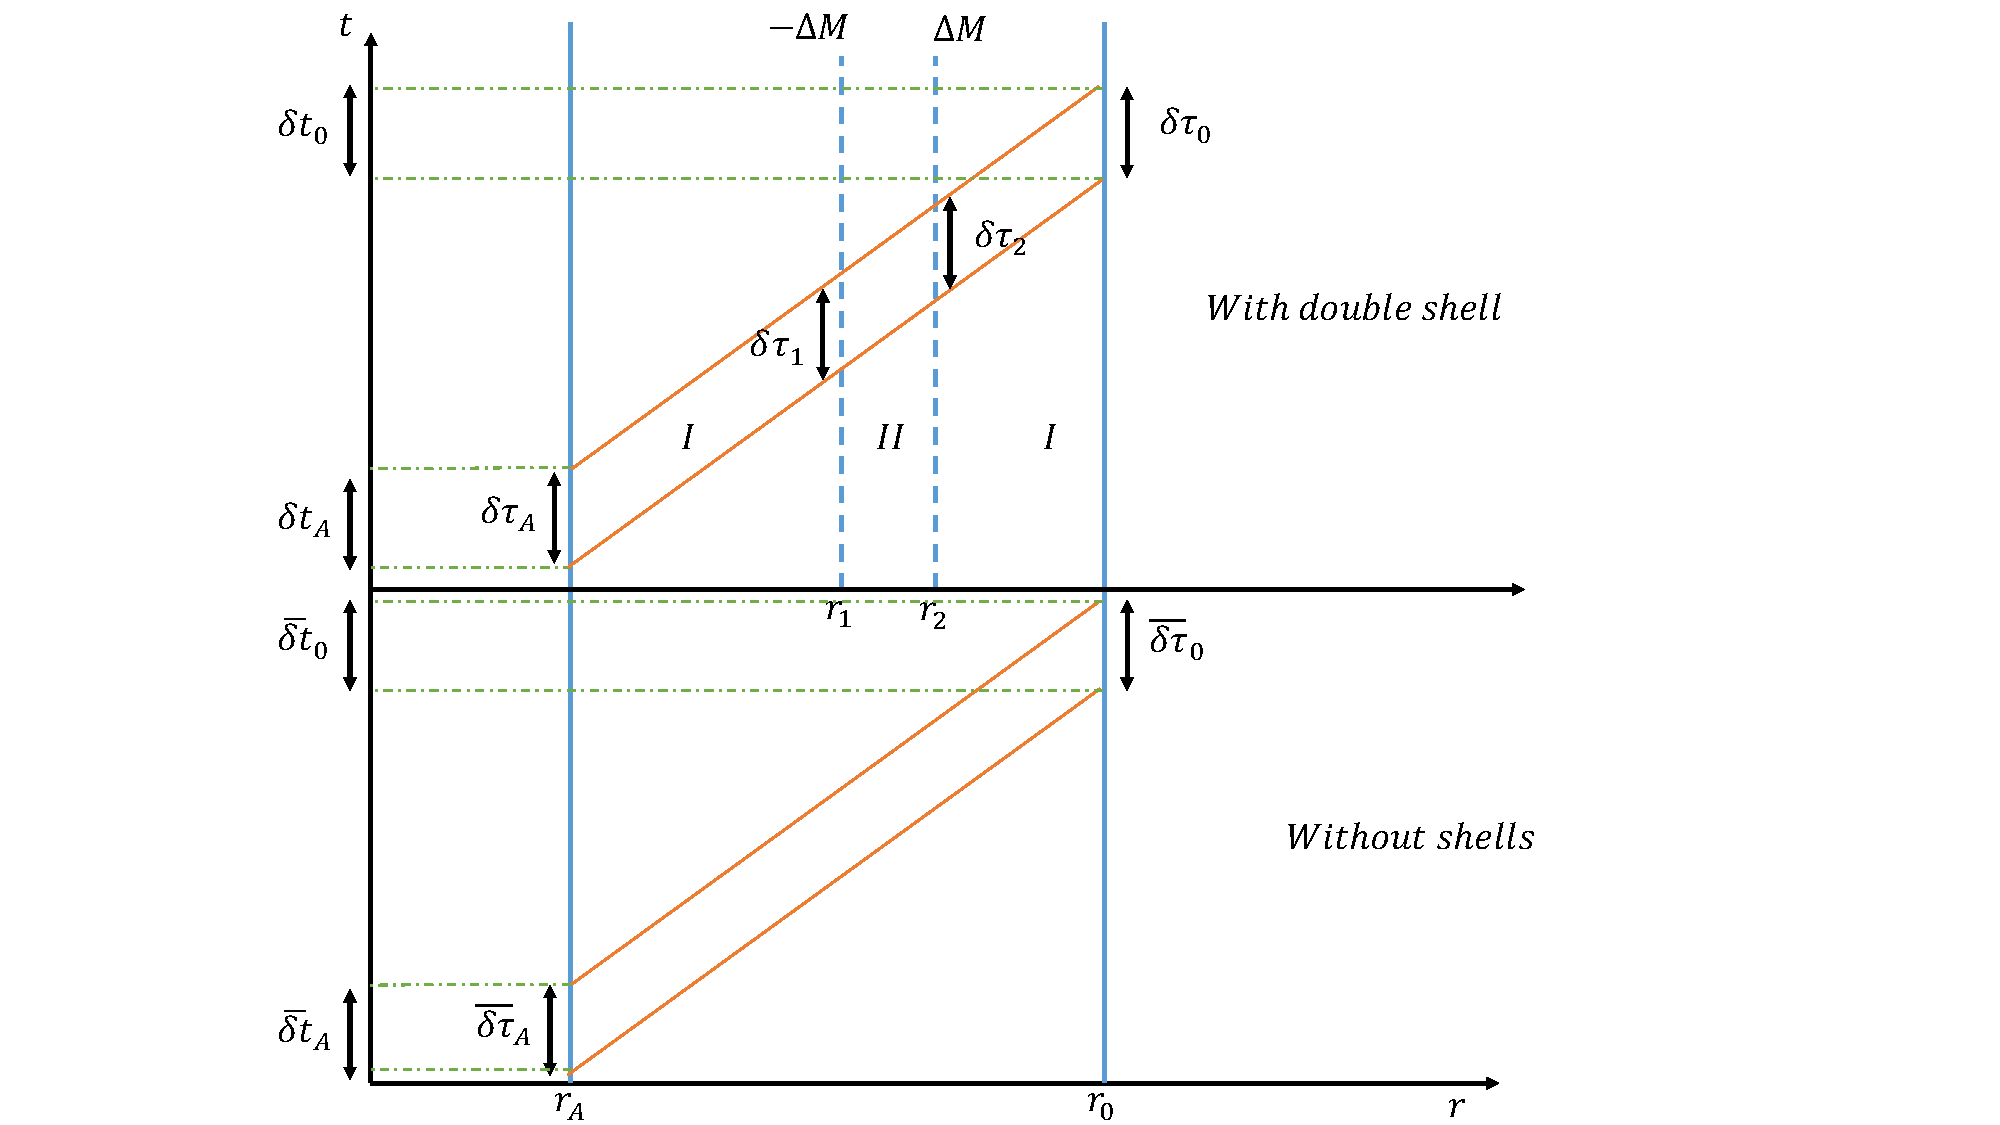
\includegraphics[height= 7 cm]{Propertime.pdf}	\label{fig:1}
%  \caption{The two parts of this diagrams describe two different scenarios. The trajectories of the photon are the lines in orange. The trajectory of the observer and the position from which the photons are emitted are represented by solid blue lines. The bottom part is a general case of two Hawking photons coming from a distance $r_A$ from the black hole of mass $M$ and arriving at an observer who is at a distance of $r_0$. The top part shows two Hawking photons coming from the same distance $r_A$ from a black hole of mass $M$. Instead of the photons freely propagating through to an observer at $r_0$, they have to cross two shells, represented by blue dotted line, of equal and opposite mass $-\Delta M, \Delta M$ at $r_{1}, r_{2}$ respectively. The regions $I$ represent a metric with mass $M$ and region $II$ represents a metric with mass $M-\Delta M$.}
%\end{SCfigure}

%\twocolumngrid

Without shells we saw that the proper time interval $\bar{\delta \tau}_0 \approx \delta t_A$, thus the difference in the proper time intervals with the shells is

\begin{equation}
	\delta \tau_0 - \bar{\delta \tau_0} = \delta t_A \left( \left( \frac{2M - r_2}{2M - r_1} \right)^\frac{1}{2} \left( \frac{ 2(\Delta M - M) + r_1}{2(\Delta M - M) + r_2} \right)^\frac{1}{2} - 1 \right). 	\label{PTD}
\end{equation}
As a check we see that when $r_1 = r_2$, $\delta \tau_0 = \bar{\delta \tau}_0$ as expected. 

We can explore this relation further by going to a region close to the horizon. If we choose $r_1 = 2M + \epsilon_1$ and $r_2 = 2M + \epsilon_2$ where $\epsilon_{1,2} <<1$, the expression in Eq (\ref{PTD}) reduces to 

\begin{equation}
	\delta \tau_0 - \bar{\delta \tau_0} = \left( \left( \frac{\epsilon_2}{\epsilon_1} \left( \frac{2\Delta M + \epsilon_1}{2 \Delta M + \epsilon_2}\right) \right)^\frac{1}{2} - 1 \right) 
\end{equation}

\subsection{Frequency of Hawking photons}

\begin{figure}[h!]
\begin{center}
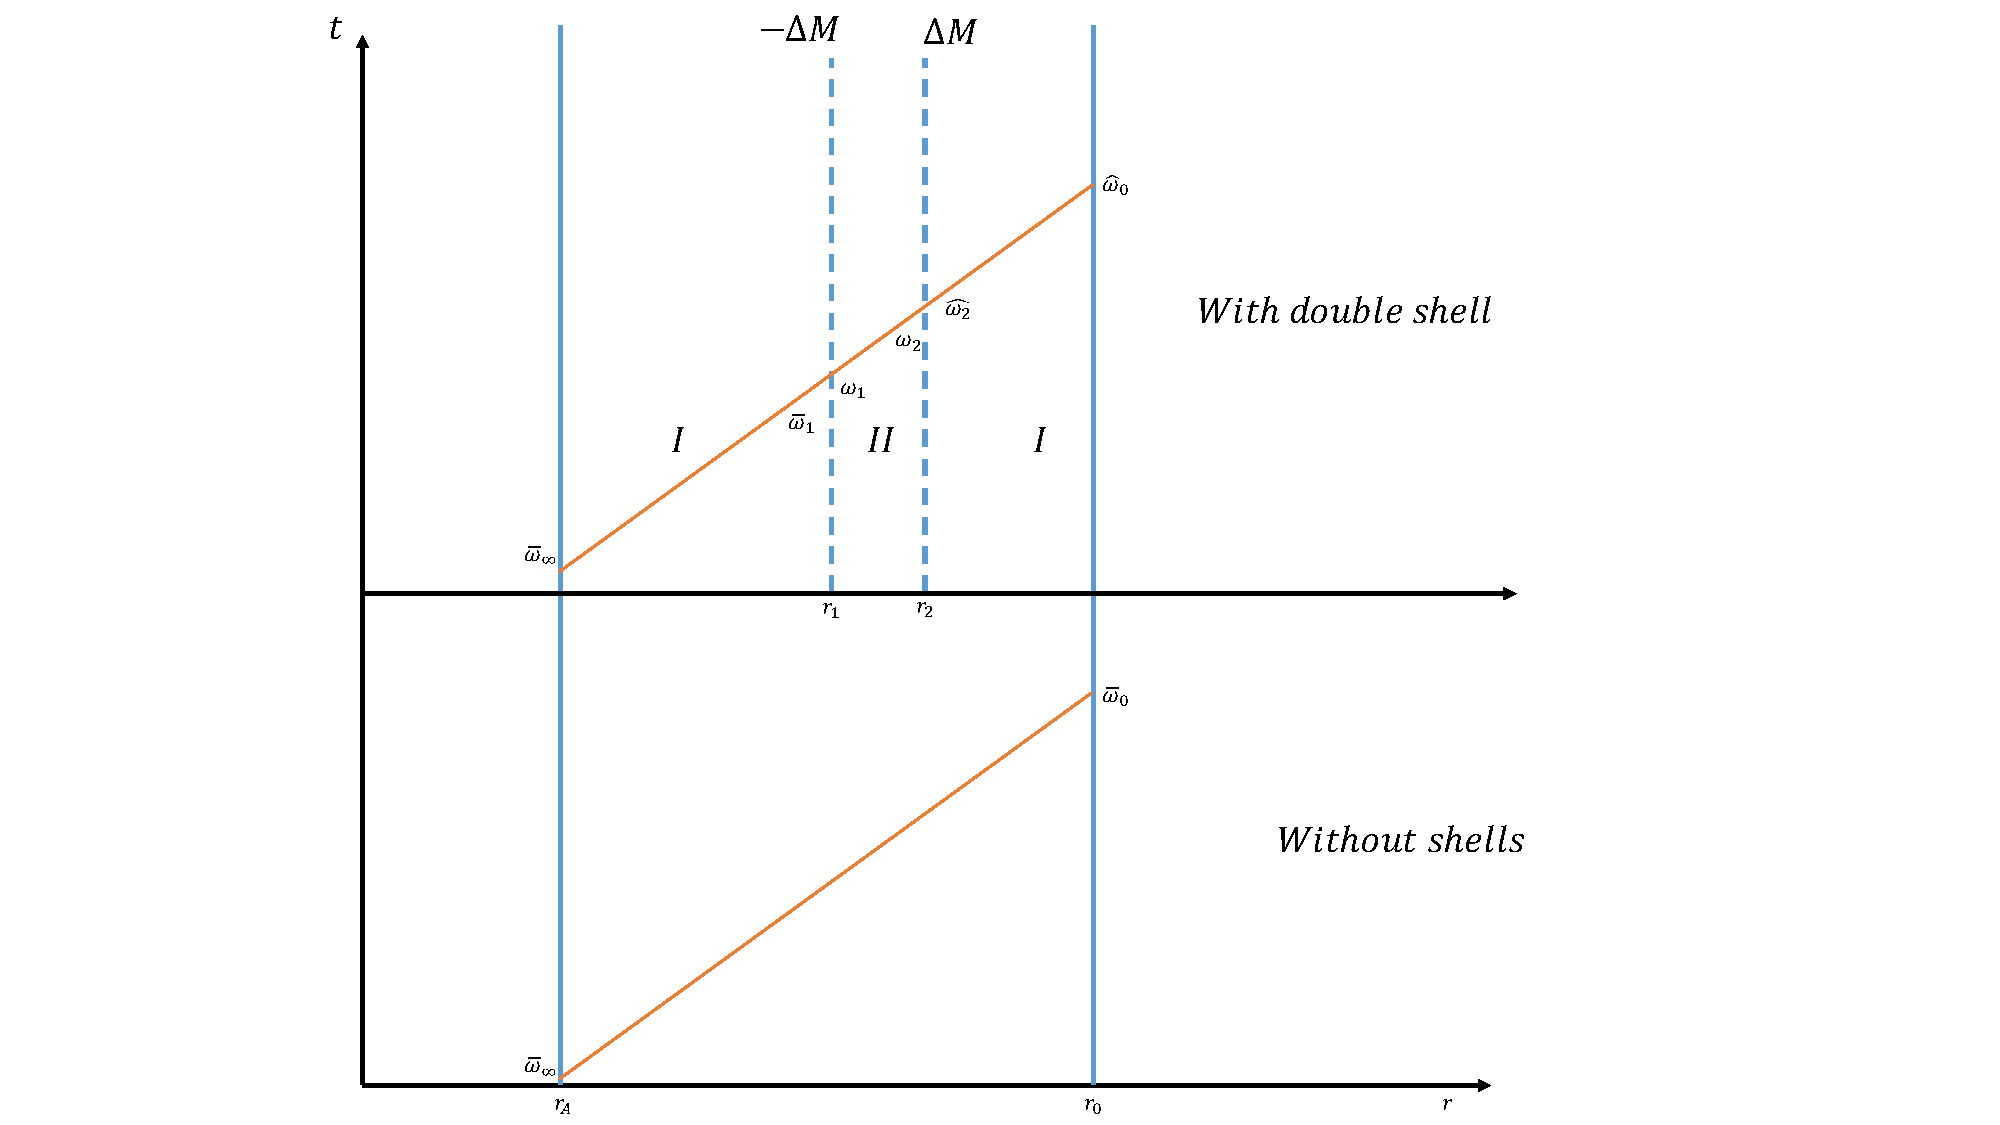
\includegraphics[scale = 0.6]{frequency.pdf}
\caption{This diagram follows the same notation as figure \ref{fig:1} except we are looking at one photon represented by the orange line. The frequency at each relevant point is denoted on the diagram. The quantities in the metric $I$ on the left of the shells are denoted with overbars. Quantities in metric $II$ are denoted without any overbars or hats. Quantities in metric $I$ to the right are denoted with hats on top.}
\label{fig:2}
\end{center}
\end{figure}


\subsubsection{Background spacetime}
We can do an analogous calculation to see this effect. Instead of looking at the proper time interval between photons we can consider the shift in frequency of single Hawking photon in the same two scenarios as were described in the previous section. We can write the photon four vector at distance $r$ as

\begin{equation}
	\bar{k}^\mu (\bar{\omega}_\infty, \bar{r}) = \bar{\omega}_\infty \left( \left( 1 - \frac{2M}{\bar{r}_A} \right)^{-1}, \sqrt{ 1 - \frac{\bar{b}^2}{\bar{r}_A^2} \left( 1 - \frac{2M}{\bar{r}_A} \right)}, \frac{\bar{b}}{\bar{r}_A^2}, 0 \right),
\end{equation}
where $\bar{\omega}_\infty$ is the frequency observed by a stationary observer at infinity and $b$ is the impact parameter of the photon. The general four velocity, $\bar{u}^\mu(\bar{r})$ of a stationary object in this geometry is

\begin{equation}
	\bar{u}^\mu(\bar{r}) = \left( \left( 1 - \frac{2M}{\bar{r}} \right)^{-\frac{1}{2}}, 0, 0, 0 \right).
\end{equation}

In the case where there are no shells, $\bar{\omega}_\infty$ is exactly the frequency observed by the observer at $\bar{r}_0$ in the limit that $\bar{r}_0 \rightarrow \infty$. In general, the frequency observed at $\bar{r}_0$, $\bar{\omega}_0$, will be redshifted

\begin{eqnarray}
	\bar{\omega}_0 & = & \bar{k}^\mu(\bar{\omega}_\infty, \bar{r}_0) \bar{u}^\nu(\bar{r}_0) \bar{g}_{\mu \nu}(\bar{r}_0) 	\nonumber	\\
	& = & - \bar{\omega}_\infty \left( 1 - \frac{2M}{\bar{r}_0} \right)^{-\frac{1}{2} }
\end{eqnarray}

of course in the limit $\bar{r}_0 \rightarrow \infty$ we get $\bar{\omega}_0 = -\bar{\omega}_\infty$. 

\subsubsection{Introducing perturbations: Double shells}

The frequency measured at $r_1$ in metric $I$, $\bar{\omega}_1$ is 

\begin{equation}
	\bar{\omega}_1 = - \bar{\omega}_\infty \left (1 - \frac{2M}{\bar{r}_1} \right)^{-\frac{1}{2}}.
\end{equation}

In metric $II$ the observed frequency $\omega_1$ is 

\begin{eqnarray}
	\omega_1 & = & g_{\mu \nu}(r_1) k^\mu(\omega_\infty, r_1) u^\nu(r_1)	\nonumber	\\
	& = & - \omega_\infty \left( 1 - \frac{2(M- \Delta M)}{r_1} \right)^{-\frac{1}{2}}.
\end{eqnarray}

Since $\omega_1$ is a physical quantity we expect it to be the same in both in metrics, $\omega_1 = \bar{\omega}_1$ and also we expect $r_1 = \bar{r}_1, r_2 = \bar{r}_2$ (since the radius of the shell corresponds to a physical sphere of radius of $r$). This gives a relation between $\omega_\infty$ and $\bar{\omega}_\infty$

\begin{equation}
	\bar{\omega}_\infty = \omega_\infty \left( 1 - \frac{2 \Delta M}{2(\Delta M  - M)+ r_1} \right)^\frac{1}{2}.	\label{13}
\end{equation}

At $r_2$ we can again equate the observed frequencies in both metrics. In this case we define the frequency observed at infinity in metric $I$ on the right side of $r_2$ as $\hat{\omega}_\infty$, i.e the photon vector in metric $I$ for $r > r_2$ is $\hat{k}$ (But we expect the four velocity of the shell to be $\bar{u}_2$). From $k^\mu(\omega_2, r_2) u^\nu(r_2) g_{\mu \nu}(r_2) = \hat{k}^\mu(\bar{r}_2) \bar{u}^\nu(\bar{r}_2) \bar{g}_{\mu \nu} (\bar{r}_2)$ we have

\begin{equation}
	\hat{\omega}_\infty = \omega_\infty \left( 1 - \frac{2 \Delta M}{2(M-\Delta M) + r_2} \right)^\frac{1}{2}.	\label{14}
\end{equation}

By combining Eq (\ref{13}) and (\ref{14}) we get 

\begin{equation}
	\hat{\omega}_\infty = \bar{\omega}_\infty \left( \frac{(2 (\Delta M - M) + r_1)(r_2 - 2M)}{(r_1 - 2M)(2(\Delta M - M) + r_2)} \right)^\frac{1}{2}
\end{equation}

The observed frequency at $r_0$, $\hat{\omega}_0$, is

\begin{eqnarray}
	\hat{\omega}_0 & = & u^\mu(r_0) k^\nu(\hat{\omega}_\infty, r_0) g_{\mu \nu}(r_0) 	\nonumber	\\
	& = & - \bar{\omega}_\infty \left( 1 - \frac{2M}{r_0} \right)^{-\frac{1}{2}}  \left( \frac{(2 (\Delta M - M) + r_1)(r_2 - 2M)}{(r_1 - 2M)(2(\Delta M - M) + r_2)} \right)^\frac{1}{2}
\end{eqnarray}

In the limit that $r_0 \rightarrow \infty$, 

\begin{equation}
	\hat{\omega}_0 = - \bar{\omega}_\infty \left( \frac{(2 (\Delta M - M) + r_1)(r_2 - 2M)}{(r_1 - 2M)(2(\Delta M - M) + r_2)} \right)^\frac{1}{2}
\end{equation}

Looking at dynamics close to the horizon, 

\begin{eqnarray}
	r_1 & = & 2M + \epsilon_1	\nonumber	\\
	r_2 & = & 2M + \epsilon_2
\end{eqnarray}

we get

\begin{equation}
	\hat{\omega}_0 = - \bar{\omega}_\infty \left( \frac{\epsilon_2}{\epsilon_1} \left( \frac{2 \Delta M + \epsilon_1}{2 \Delta M + \epsilon_2} \right) \right)^\frac{1}{2}
\end{equation}
















\bibliography{all_active}


\end{document}